\documentclass[chi]{sigchi}

% Use this section to set the ACM copyright statement (e.g. for
% preprints).  Consult the conference website for the camera-ready
% copyright statement.

% Copyright
\CopyrightYear{2019}
%\setcopyright{acmcopyright}
\setcopyright{acmlicensed}
%\setcopyright{rightsretained}
%\setcopyright{usgov}
%\setcopyright{usgovmixed}
%\setcopyright{cagov}
%\setcopyright{cagovmixed}
% DOI
\doi{http://dx.doi.org/10.475/123_4}
% ISBN
\isbn{123-4567-24-567/08/06}
%Conference
\conferenceinfo{ASSETS'19,}{October 28--30, 2019, Pittsburgh, Pennsylvania}
%Price
\acmPrice{\$15.00}

% Use this command to override the default ACM copyright statement
% (e.g. for preprints).  Consult the conference website for the
% camera-ready copyright statement.

%% HOW TO OVERRIDE THE DEFAULT COPYRIGHT STRIP --
%% Please note you need to make sure the copy for your specific
%% license is used here!
% \toappear{
% Permission to make digital or hard copies of all or part of this work
% for personal or classroom use is granted without fee provided that
% copies are not made or distributed for profit or commercial advantage
% and that copies bear this notice and the full citation on the first
% page. Copyrights for components of this work owned by others than ACM
% must be honored. Abstracting with credit is permitted. To copy
% otherwise, or republish, to post on servers or to redistribute to
% lists, requires prior specific permission and/or a fee. Request
% permissions from \href{mailto:Permissions@acm.org}{Permissions@acm.org}. \\
% \emph{CHI '16},  May 07--12, 2016, San Jose, CA, USA \\
% ACM xxx-x-xxxx-xxxx-x/xx/xx\ldots \$15.00 \\
% DOI: \url{http://dx.doi.org/xx.xxxx/xxxxxxx.xxxxxxx}
% }

% Arabic page numbers for submission.  Remove this line to eliminate
% page numbers for the camera ready copy
% \pagenumbering{arabic}

% Load basic packages
\usepackage{balance}       % to better equalize the last page
\usepackage{graphics}      % for EPS, load graphicx instead 
\usepackage[T1]{fontenc}   % for umlauts and other diaeresis
\usepackage{txfonts}
\usepackage{mathptmx}
\usepackage[pdflang={en-US},pdftex]{hyperref}
\usepackage{color}
\usepackage{xspace}
\usepackage{booktabs}
\usepackage{textcomp}

% Some optional stuff you might like/need.
\usepackage{microtype}        % Improved Tracking and Kerning
% \usepackage[all]{hypcap}    % Fixes bug in hyperref caption linking
\usepackage{ccicons}          % Cite your images correctly!
% \usepackage[utf8]{inputenc} % for a UTF8 editor only

% If you want to use todo notes, marginpars etc. during creation of
% your draft document, you have to enable the "chi_draft" option for
% the document class. To do this, change the very first line to:
% "\documentclass[chi_draft]{sigchi}". You can then place todo notes
% by using the "\todo{...}"  command. Make sure to disable the draft
% option again before submitting your final document.
\usepackage{todonotes}

% Paper metadata (use plain text, for PDF inclusion and later
% re-using, if desired).  Use \emtpyauthor when submitting for review
% so you remain anonymous.
\def\plaintitle{Leveraging Augmented Reality to Create Apps for People with Visual Disabilities: A Case Study in Indoor Navigation}
\def\plainauthor{First Author, Second Author, Third Author,
  Fourth Author, Fifth Author, Sixth Author}
\def\emptyauthor{}
\def\plainkeywords{orientation and mobility; augmented reality; assistive tech}
\def\plaingeneralterms{Documentation, Standardization}

% llt: Define a global style for URLs, rather that the default one
\makeatletter
\def\url@leostyle{%
  \@ifundefined{selectfont}{
    \def\UrlFont{\sf}
  }{
    \def\UrlFont{\small\bf\ttfamily}
  }}
\makeatother
\urlstyle{leo}

% To make various LaTeX processors do the right thing with page size.
\def\pprw{8.5in}
\def\pprh{11in}
\special{papersize=\pprw,\pprh}
\setlength{\paperwidth}{\pprw}
\setlength{\paperheight}{\pprh}
\setlength{\pdfpagewidth}{\pprw}
\setlength{\pdfpageheight}{\pprh}

% Make sure hyperref comes last of your loaded packages, to give it a
% fighting chance of not being over-written, since its job is to
% redefine many LaTeX commands.
\definecolor{linkColor}{RGB}{6,125,233}
\hypersetup{%
  pdftitle={\plaintitle},
% Use \plainauthor for final version.
%  pdfauthor={\plainauthor},
  pdfauthor={\emptyauthor},
  pdfkeywords={\plainkeywords},
  pdfdisplaydoctitle=true, % For Accessibility
  bookmarksnumbered,
  pdfstartview={FitH},
  colorlinks,
  citecolor=black,
  filecolor=black,
  linkcolor=black,
  urlcolor=linkColor,
  breaklinks=true,
  hypertexnames=false
}



\newcommand{\BVI}{B/VI\xspace}
\newcommand{\OM}{O\&M\xspace}


% create a shortcut to typeset table headings
% \newcommand\tabhead[1]{\small\textbf{#1}}

% End of preamble. Here it comes the document.
\begin{document}

\title{\plaintitle}

\numberofauthors{3}
\author{%
  \alignauthor{Chris Yoon\\
    \affaddr{Stanford University}\\
    \affaddr{Palo Alto, USA}\\
    \email{csyoon95@stanford.edu}}\\
              \alignauthor{Ryan Louie, Jeremy Ryan, MinhKhang Vu, Hyegi Bang, William Derksen\\
    \affaddr{Olin College of Engineering}\\
    \affaddr{Needham, USA}\\
    \email{\{ryan.louie, jeremy.ryan, minhkhang.vu, hyegi.bang, william.derksen\}@students.olin.edu}}\\
    \alignauthor{Paul Ruvolo\\
    \affaddr{Olin College of Engineering}\\
    \affaddr{Needham, USA}\\
    \email{paul.ruvolo@olin.edu}}\\
}

\maketitle

\begin{abstract}
The introduction of augmented reality technology to iOS and Android enables, for the first time, mainstream smartphones to estimate their own motion in 3D space with high accuracy.  For assistive technology researchers, this development presents a potential opportunity.  In this spirit, we present our work leveraging these technologies to create a smartphone app to empower people who are visually impaired to more easily navigate indoor environments.  Our app, \emph{Clew}, allows users to record routes and then load them, at any time, providing automatic guidance (using haptic, speech, and sound feedback) along the route.  We present our user-centered design process, Clew's system architecture and technical details, and both small and large-scale evaluations of the app.  We discuss opportunities, pitfalls, and design guidelines for utilizing augmented reality for orientation and mobility apps.  Our work expands the capabilities of technology for orientation and mobility that can be distributed on a mass scale.
\end{abstract}

\category{K.4.2.}{Assistive technology for persons with disabilities}{Orientation and mobility tools for persons with visual disabilities}

\keywords{\plainkeywords}
\section{Introduction}
For people who are blind or visually impaired (\BVI), improvements in orientation and mobility (\OM) have been shown to increase economic opportunity as well as psychological well-being.  While only 30\% of working-age Americans who are \BVI are employed \cite{employmentstatistics2017, kirchner1999looking}, those who have better \OM skills have higher rates of employment \cite{crudden1998comprehensive, crudden1999barriers, leonard1999factors, o1999employment}.

The mobility cane is the most widely used tool for \OM and serves as the foundation upon which most \OM skills are built \cite{wiener2010foundations}.  Among its many functions, the mobility cane helps people who are \BVI to sense and interpret spatial information (e.g., the location of ground-level obstacles and landmarks).  The detection of salient elements in the environment and their spatial relationships helps people who are \BVI to maintain their personal safety, form mental maps of their surroundings, and orient themselves within an environment \cite{thinus1997representation, schinazi2016spatial}.

Despite its many virtues, the mobility cane does not adequately address all aspects of \OM.  As a result, there is a long history of work to develop assistive technologies that augment the capabilities of the mobility cane \cite{wiener2010foundations}.  For instance, several projects were undertaken to create high-tech versions of the mobility cane that provide enhanced obstacle detection capabilities \cite{benjamin1973new, borenstein1997guidecane}.  Well before such technology entered the mainstream, there was  work to create assistive devices to help with navigation and route planning \cite{dakopoulos2010wearable}.  Despite considerable efforts, few of these technologies have achieved much impact beyond the lab \cite{wiener2010foundations}.  In part, this lack of impact has been driven by the fact that the technologies were expensive, unreliable, cumbersome, or hard to distribute on a mass scale.

One notable exception to this disappointing track record is GPS navigation apps for smartphones.  Since these apps are built using mainstream technologies that happen to be universally accessible --- as opposed to special purpose assistive technologies --- they are robust, powerful, and useful to people who are \BVI.  Further, the fact that a majority of people who are \BVI own smartphones \cite{morris2014blind} makes them distributable at either no additional cost (e.g., Google Maps) or at modest cost (e.g., BlindSquare, which is designed for people who are \BVI and costs about \$30).

Despite the undeniable impact of smartphone-based GPS technology, importantly, mass market GPSes are only accurate to about $5m$ under open sky (and are even worse in challenging environments such as cities) and do not work indoors.  The need for technology to assist with \OM tasks that go beyond outdoor navigation (e.g., to enable indoor navigation or improved mental mapping of one's environment) has been well-documented \cite{long1997establishing}.  As such, due to GPS's limitations, there is a need to investigate alternative technologies.  Many researchers have worked to address these challenges and provide solutions that increase access for people who are \BVI to physical spaces (see \emph{Related Work}).

One particularly promising technology for addressing \OM challenges is augmented reality (AR).  Recently, smartphone manufacturers have introduced AR modules that support high-accuracy 3D-tracking.  While the primary purpose of these modules is to enable AR experiences --- whereby virtual and physical content are mingled, e.g., by overlaying virtual characters on a smartphone's camera feed --- these modules have the potential to be repurposed to create assistive technology for \OM that is high-precision and usable indoors.  Further, since AR is now a standard feature of smartphones, \OM apps that use AR can be widely distributed at no cost.

With the significant potential of smartphone-based AR technology comes critical research questions.  Are the motion estimates provided robust enough to use for \OM? If so, which \OM tasks might be facilitated?  What usability challenges does AR technology bring, and how can we, as designers, best support users in harnessing such technology?  Here, we take preliminary steps towards answering these questions by presenting our work utilizing user-centered design to leverage the AR modules in modern smartphones to create, and to release to a global audience, an application to assist with indoor navigation.  Our app, \emph{Clew}, enables users to record routes using their smartphone so that they can later navigate these routes with automatic guidance.  Clew is designed to alleviate various pain points experienced by people who are \BVI (e.g., finding one's way back after being guided to a location or following a new route in an unfamiliar environment).%  Our experiences designing, implementing, and deploying \emph{Clew} provide both quantitative and qualitative information towards answering these research questions.%  In order to design maximally impactful technologies, we employ user-centered design principles throughout our research and development process.%  Specifically, we worked longitudinally with co-designers who are \BVI and two of the study authors, who are visually impaired themselves, contributed to all aspec	ts of the project and provided design guidance based on their personal experiences.

In the remainder of the paper we review some of the existing research on \OM assistive technology, discuss the algorithms that underlie AR technology on smartphones, present the design of Clew, provide small- and large-scale evaluations of Clew, and discuss future challenges and promising directions for smartphone-based AR technology for people who are \BVI.

\section{Related work}


A number of researchers have worked to overcome the limitations (e.g., less-than-ideal accuracy, lack of availability indoors) of GPS technology for assisting people who are \BVI with \OM.  One approach is to utilize crowdsourcing, whereby people who are \BVI connect over the internet with a sighted person for real-time assistance.  Examples of this approach include the VizWiz project \cite{bigham2010vizwiz}, BeMyEyes \cite{bemyeyesaccessworld}, and Aira \cite{aira} (both BeMyEyes and Aira support a video chat interface).  A second approach combines noisy motion estimates derived from inertial sensors (gyroscopes and accelerometers) with either detection of fixed environmental infrastructure (e.g., Bluetooth beacons, Wifi access points, infrared emitters, signs \cite{legge2013indoor}) or imposition of prior knowledge of the environment to reduce motion tracking drift \cite{riehle2013indoor}.  For instance, Ganz and colleagues developed a system for navigation using smartphone-detectable RFID tags \cite{ganz2015percept, ganz2011percept, ganz2014percept}.  Dias and her collaborators utilized WiFi fingerprinting and dead-reckoning for indoor navigation \cite{Dias__2014_7778}, and similar systems based on Bluetooth beacons have also been developed \cite{ishihara2017beacon, ahmetovic2016navcog}.  Others have explored the use of robots as guides for people who are blind \cite{Nanavati:2018:CIN:3173386.3176976}.%\todo{Generally need to expand on this given that we are not trying to hit the 5-page limit. More detail can be added as well as incorporating some of the references from my 2018 CAREER submission.}

There is some work on recording and retracing routes in unmodified indoor environments.  In \cite{flores2018easy, flores2014ariadne}, Flores and Manduci present a system that counts steps (for estimating linear motion) and detects 90-degree turns to first record and then to retrace a route.  In \cite{fusco2018indoor}, the authors present a localization system based on combining AR-based tracking and sign recognition.  The authors found satisfactory localization performance of their system for two of the test users and poor performance for the third as measured along three indoor routes (localization information was translated into navigation guidance using a Wizard-of-Oz approach).  In comparison, the novelty of our work lies in support of route saving and reloading while making minimal assumptions about the environment (e.g., the availability of signs for tracking or that all turns are 90 degrees), a large-scale evaluation of our app, and the generation of specific design guidelines for researchers who would like to incorporate AR technology into \OM applications.

%Another area of research is the development of solutions to help people who are \BVI find objects that were misplaced, moved by a third party, or whose locations were never known.  While the task of object finding doesn't fall under the umbrella of \OM, here we stretch the terminology to encompass it by noting that both \OM and object finding require a significant degree of spatial awareness.  As in the case of navigation, crowdsourcing approaches have shown promise for object finding \cite{bigham2010vizwizlocateit}.  Other approaches use automatic object detection and tracking to navigate to objects \cite{schauerte2012assistive, jafri2014computer, thakoor2014system}.%\todo{might need to explicitly contrast with our work, why is ours better, or just say that we will discuss this later}

\section{Augmented Reality}
%
%\begin{figure}
%\begin{center}
%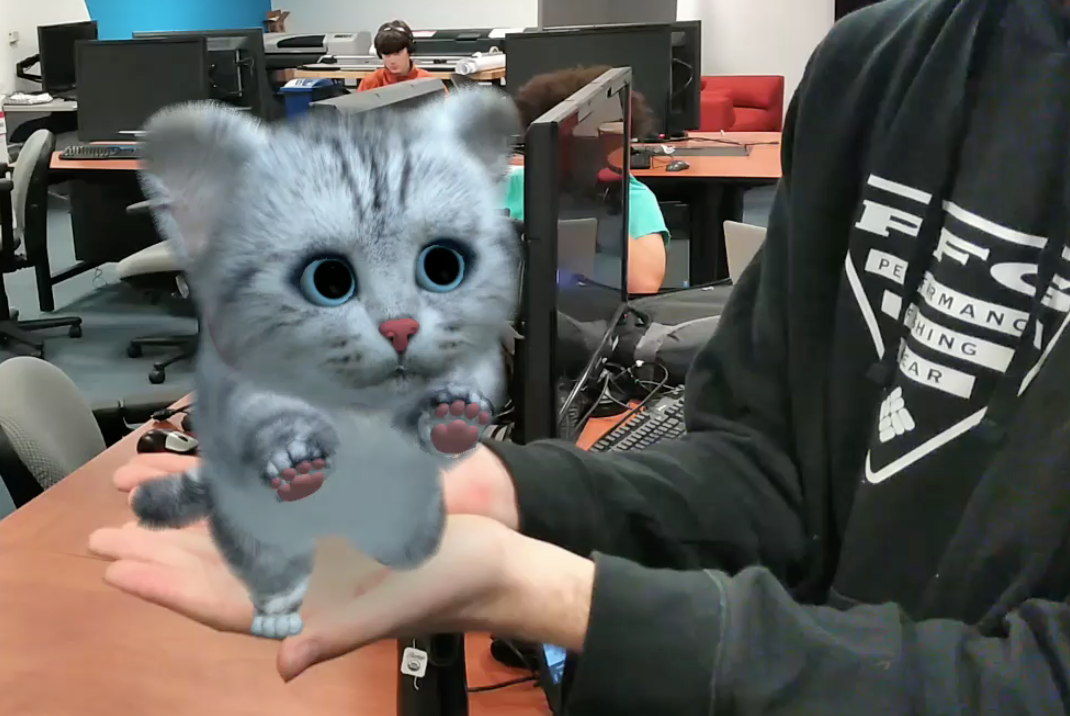
\includegraphics[width=.9\linewidth]{Figures/arexample.png}
%\end{center}
%\caption{A virtual cat overlaid on a smartphone camera feed.  The phone is able to accurately sense its movement in order to render the cat at the appropriate viewing angle and depth.\label{fig:arexample}}
%\end{figure}

Both Apple and Google have released support for smartphone-based AR experiences, whereby virtual and real content are combined.  For instance, an app might show a virtual cat projected into a real-world scene.  As the user moves, the phone senses the user's motion and renders the cat at an appropriate distance and angle, providing the illusion that the cat exists in the physical world.

These AR systems utilize 3D motion-tracking algorithms that combine data from inertial sensors (gyroscopes and accelerometers) with visual information (obtained from the phone's camera) to generate motion estimates that are far more accurate than what could be obtained using only inertial sensing.  The high accuracy of these systems is enabled by two key trends: the development of sophisticated algorithms for visual-inertial odometry (VIO) \cite{li2013high,leutenegger2015keyframe,bloesch2015robust,forster2014svo} (which are the algorithms that enable the combination of optical and inertial data for motion estimation) and the development of special-purpose hardware to allow computationally intensive algorithms to run with minimal heat generation and power consumption.%  The combination of high accuracy and low power consumption provides the motivation for the exploration of the potential of AR technology for creating \OM apps for people who are \BVI.

\subsection{Algorithms for Visual Inertial Odometry}
While a full explanation of VIO \cite{gui2015review} is beyond the scope of this paper, it helps to have a conceptual understanding of VIO.  VIO algorithms are designed for either the monocular (single camera) or stereo setting.  Since the monocular setting is the one currently applicable to mass-market smartphones, here we use the term VIO to refer to monocular VIO specifically.

VIO algorithms blend optical and inertial motion estimates.  Optical motion estimates are made by tracking salient visual features --- e.g., corners or other textured portions of an image --- through multiple video frames.  Utilizing the mathematics of perspective geometry, one can estimate the rotation and translation of the camera \cite{Hartley2004}.  Importantly, the accuracy of these estimates is dependent on tracking a large number of visual features that should, ideally, correspond to points at a range of depths from the camera.%  While some environments are intrinsically more difficult for optical tracking, we have observed that users may exacerbate this difficulty by holding their phones in a suboptimal orientation (e.g., with the camera facing the ground).

Further complicating matters, the translation estimated using optical tracking is only determined up to an arbitrary scale factor.  This indeterminacy arises due to the fact that the depths of the tracked visual features are unknown \cite{Hartley2004}.  For example, given an estimate of the translation of a camera, it is possible that the camera moved twice as far and the depths of the tracked points were twice as great.  The shortcomings of optical tracking, scale-indeterminacy and inaccurate performance in feature-poor environments, can be overcome by the fusion of inertial measurements from gyroscopes and accelerometers.  Gyroscopes, which provide accurate estimates of angular velocity, can refine estimates of rotation while accelerometer data can be integrated over time to obtain estimates of linear velocity, overcoming the scale-indeterminacy problem.

\subsection{VIO in Mass-Market Smartphones}
Both Apple and Google have released AR modules based on VIO.  While the details of their algorithms are not publicly available, there are distinctions between these frameworks that researchers should keep in mind.

\subsubsection{Google Tango}
Release in late 2014 by Google's ATAP (Advanced Technology and Projects) division, Tango utilizes a wide-angle, fisheye lens and a global image shutter to enable accurate visual-feature tracking.  The platform also includes a PrimeSense depth-sensing camera.  Two commercial smartphones have been released based on the Tango platform: the Lenovo Phab2 Pro and the Asus Zenfone AR.  While the tracking capabilities of Tango devices are superior to both ARKit and ARCore (discussed next), the reliance on special-purpose cameras severely limited the adoption of the technology.  As a result, Google suspended the project in early 2018 \cite{tangoretired}.


\subsubsection{ARKit and ARCore}
\begin{figure*}
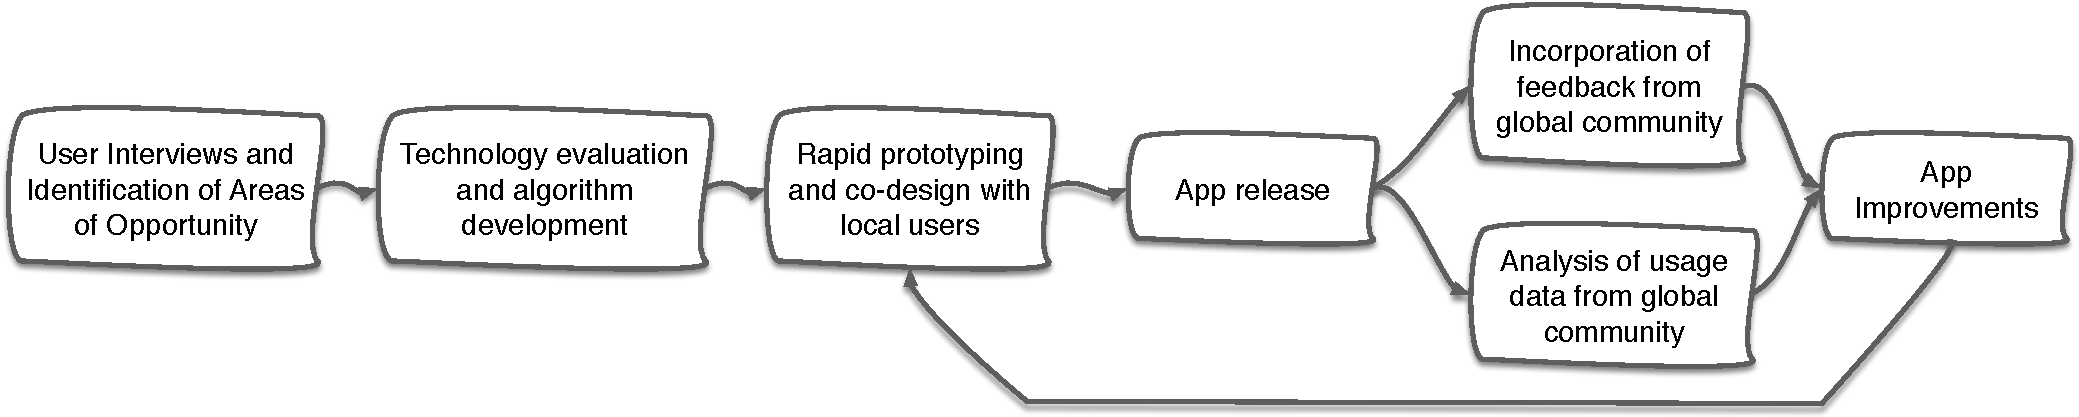
\includegraphics[width=\linewidth]{Figures/designprocess}
\caption{Our design process used to investigate the usage of AR technology for creating assistive technologies for people who are \BVI.  We are using this process to design our app \emph{Clew}.\label{fig:designprocess}}
\end{figure*}
Apple's ARKit \cite{arkit}, released in 2017, and Google's ARCore \cite{arcore}, released in 2018, do not require special-purpose cameras.  Since these platforms utilize conventional cameras, which have comparatively limited fields-of-view when compared to a fisheye camera, the richness of visual features available for tracking is not as great as with Tango.  Consequently, motion estimates are less accurate.  Further, since neither of these platforms have depth-sensing cameras, the availability of 3D information is limited to objects with special structure (e.g., horizontal and vertical planar surfaces).  Despite their drawbacks, these frameworks can run on a wider array of phones than Tango, and given the large preference for iOS among people who are \BVI \cite{morris2014blind}, ARKit is the primary platform of interest for researchers seeking to develop \OM apps for people who are \BVI.

%Although quite specific and certainly at the implementation detail level, a challenge presented when developing assistive apps for ARKit is that the ARSCNView class provided by Apple does not allow for the presentation of subviews.  This limitation makes it particular hard to achieve optimal integration with Apple's VoiceOver.  In particular, it is very difficult to make an app that consistently announces the identity of activated buttons, while also properly announcing new controls that appears on the screen.

\section{Design Process Overview}
\begin{table}
  \centering
  \begin{tabular}{c c c c}
    % \toprule
    {\small \textit{Pseudonym}}
            & {\small \textit{Gender}} & {\small \textit{Proficiency with smartphones}} & {\small \textit{Means of \OM}} \\
    \midrule
    Joe  & male  & medium & dog \\
    Carmen  &  male & high & cane \\
   Karen  & female & high & cane\\
    George  & male & low & cane
    % \bottomrule
  \end{tabular}
  \caption{Some of the attributes of the co-designers who helped create the Clew app.  Each co-designer visited Olin five times for roughly three hours per session.\label{tab:codesigners}}
\end{table}

We employed a user-centered design process that involves people who are \BVI in all phases (see Figure~\ref{fig:designprocess}).  In the initial phase, we focused on in-person interactions with members of the greater-Boston \BVI community and members of the research team who are \BVI to identify areas of opportunity for improving access to physical spaces (see \emph{\nameref{sec:areasofopportunity}}).  Based on these interactions, we developed concepts for \OM apps.  These app concepts fed into a co-design process.  Each co-designer visited Olin College weekly over a period of five weeks for roughly three hours per session.  In total, we interacted with four co-designers (three male and one female) in this fashion.  Each co-designer had minimal functional vision and relied on non-visual means for \OM.  Some basic attributes of our co-designers, and their pseudonyms are presented in Table~\ref{tab:codesigners}.  Over the course of these co-designs we created system architectures, selected and developed algorithms, and ultimately produced prototype apps, which our partners engaged with (see \emph{\nameref{sec:areasofopportunity}}).  We iterated this design cycle based on feedback from our co-designers.

Once we had an app that was polished as well as useful to the \BVI community, we released the app on the iOS App Store.  The release of the app generated feedback in two forms.  First, users from all over the world gave us their impressions of the app and how they would want to see it improved.  Second, users who opted-in to sharing usage data, provided a dataset to understand, in a quantitative manner, how the app was being utilized (see \emph{\nameref{sec:largescalestudy}}).

\subsection{User Interviews and Areas of Opportunity}\label{sec:areasofopportunity}
Our earliest co-design partner was Joe (pseudonym), a college student with no functional vision due to Retinitis Pigmentosa (a degenerative vision disorder that leads to the breakdown of cells in the retina).  Joe is a non-visual traveler, mostly navigating with the help of his guide dog (see Table~\ref{tab:codesigners}). We also talked at length with an \OM trainer for primary and middle school students who shared stories of mobility challenges that his students face. Furthermore, three members of our research team, two of whom are low-vision and one of whom is blind, contributed to the design and implementation of the app and leveraged their personal experiences and knowledge of the \BVI community to inform this work.  Our team identified a number of pain points and areas of opportunity related to \OM and access to physical spaces.

\textbf{Navigating in unfamiliar indoor environments is difficult.} In these situations, one will often need to either ask a sighted person to assist them or bring along a sighted friend or family member.  If one will be navigating this environment over a long period of time, for instance when starting a new job, one may work with a mobility instructor to learn how to navigate this new environment.  A common sentiment among our co-designs was that relying on others for assistance in these scenarios is a major impediment to independence.

\textbf{Navigating newly traveled routes towards previously visited locations is difficult.} A specific subset of the difficulties encountered in navigating new indoor environments is navigating back to a starting point after traveling to a new location.  As an example, a member of our design team expressed that finding his seat (e.g., in a classroom) after going to the restroom was challenging.  A second example is that one of our visually impaired team members found it difficult to find his seat on a dimly lit airplane when returning from the restroom.

The identification of these pain points motivated the creation of Clew to support indoor navigation in unfamiliar environments.%  In \emph{\nameref{sec:clewoverview}}, we present the app's features and technical architecture.%  In \emph{\nameref{sec:usabilityandevaluation}}, we present both small and large-scale studies that provide insight into the app's capabilities, suggest improvements to its design, and provide guidelines for developers of similar apps.

\section{Clew App Overview}\label{sec:clewoverview}

\begin{figure*}
\begin{center}
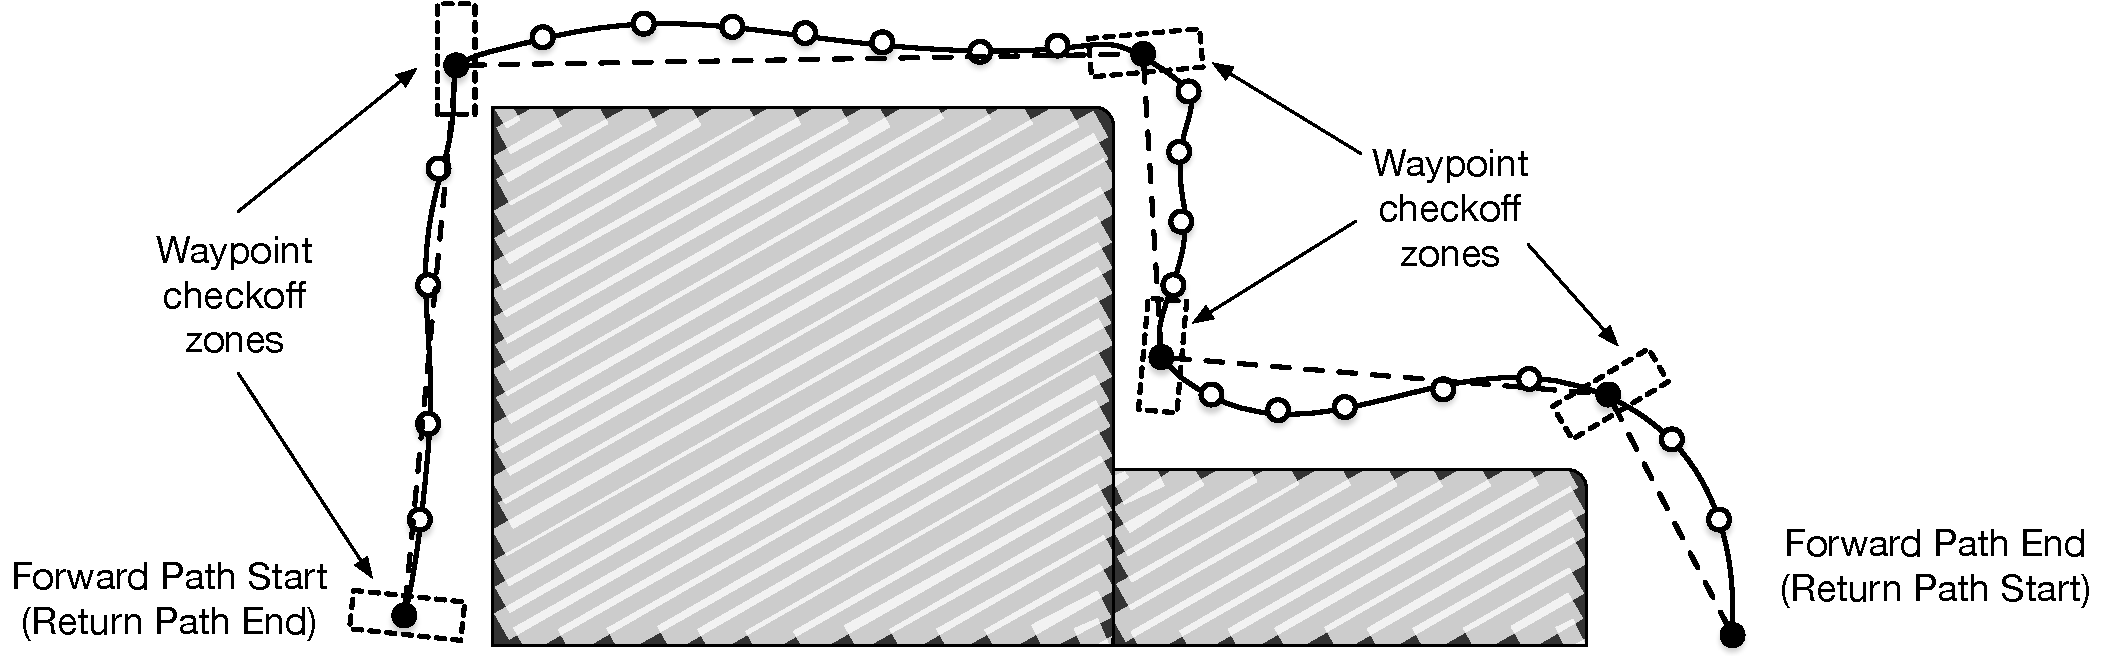
\includegraphics[width=\linewidth]{Figures/samplepath}
\end{center}
\caption{A top-down view of a path generated by the \emph{Clew}.  The figure shows the raw path (solid line) and breadcrumbs (white circles with black outlines).  The Ramer-Douglas-Peucker algorithm is applied to reduce the breadcrumbs to a more manageable number of waypoints (solid black circles).  The resultant path consists of straight lines connecting these waypoints in reverse order.  Waypoint checkoff zones are shown as dashed boxes.\label{fig:samplepath}}
\end{figure*}

Clew is an iOS app that provides continuous guidance to users who are \BVI as they travel along pre-recorded routes.  The app serves two main use cases.  The first use case is to allow the user to record a path through an indoor environment and then navigate the path back to the starting location.  One situation where this use case arises is when a user is led somewhere by a sighted guide and they want to return to their previous location --- without being guided back.  A second situation where this use case can arise is when it is easier to navigate from a location than back to it (e.g., it is easier for someone who is \BVI to leave a conference room than it is to find their way back to their particular seat).  The second use case is to allow the user to record a path through an indoor environment, save this path, and then navigate the path either in the forward or reverse direction at a later point in time.  This function is useful when a user is either learning to navigate a route and could use guidance (e.g., when practicing) or when the user wants to navigate a new route repeatedly for a brief period of time (e.g., during a hotel stay a user may want to navigate to their room or to the hotel pool).

In order to serve each of these use cases, Clew provides the core functionality of route recording along with high-accuracy, easy-to-follow, navigational guidance to enable people who are \BVI to travel independently indoors.%, without the need for modifications to the environment (e.g., the introduction of beacons or special signage).

\subsection{Path Recording}

In path recording mode, the app lays down a trail of virtual breadcrumbs (representing timestamped, 3D positions and orientations) while the user traverses a route.  These estimates of position and orientation are generated by Apple's ARKit, which provides these at a rate of 60 Hz.  Recall that these position and orientation estimates are based on fusing visual and inertial motion measurements. % RatheWe record the phone's position every $300$ milliseconds to tradeoff computational constraints with faithfully representing the travelled route,

Once the user starts recording, they travel to a new location (either via their traditional \OM process or via assistance from a sighted guide) and then stops the recording.  Figure~\ref{fig:samplepath} shows a sample path along with virtual breadcrumbs.
%
\subsection{Route Pausing and Saving through Landmark Creation}

ARKit tracks motion in a coordinate system whose origin coincides with the device's position when the app starts.  Thus the positions of any breadcrumbs dropped during the path recording phase are meaningful only \emph{within} the context of the current ARKit tracking session.  Once a path is recorded, if the user doesn't switch to a different app, lock the phone, or occlude the camera, then they can navigate back to their starting location using the procedures described in \emph{\nameref{sec:pathnavigationmode}}.  However, if the user wishes to wait a significant amount of time before navigating back, would like to use another app, or if the user would like to save the route for use at a later time, these limitations can be prohibitive.  In order to support such cases, Clew provides support for route pausing and saving through coordinate system registration.


\begin{figure}
\begin{center}
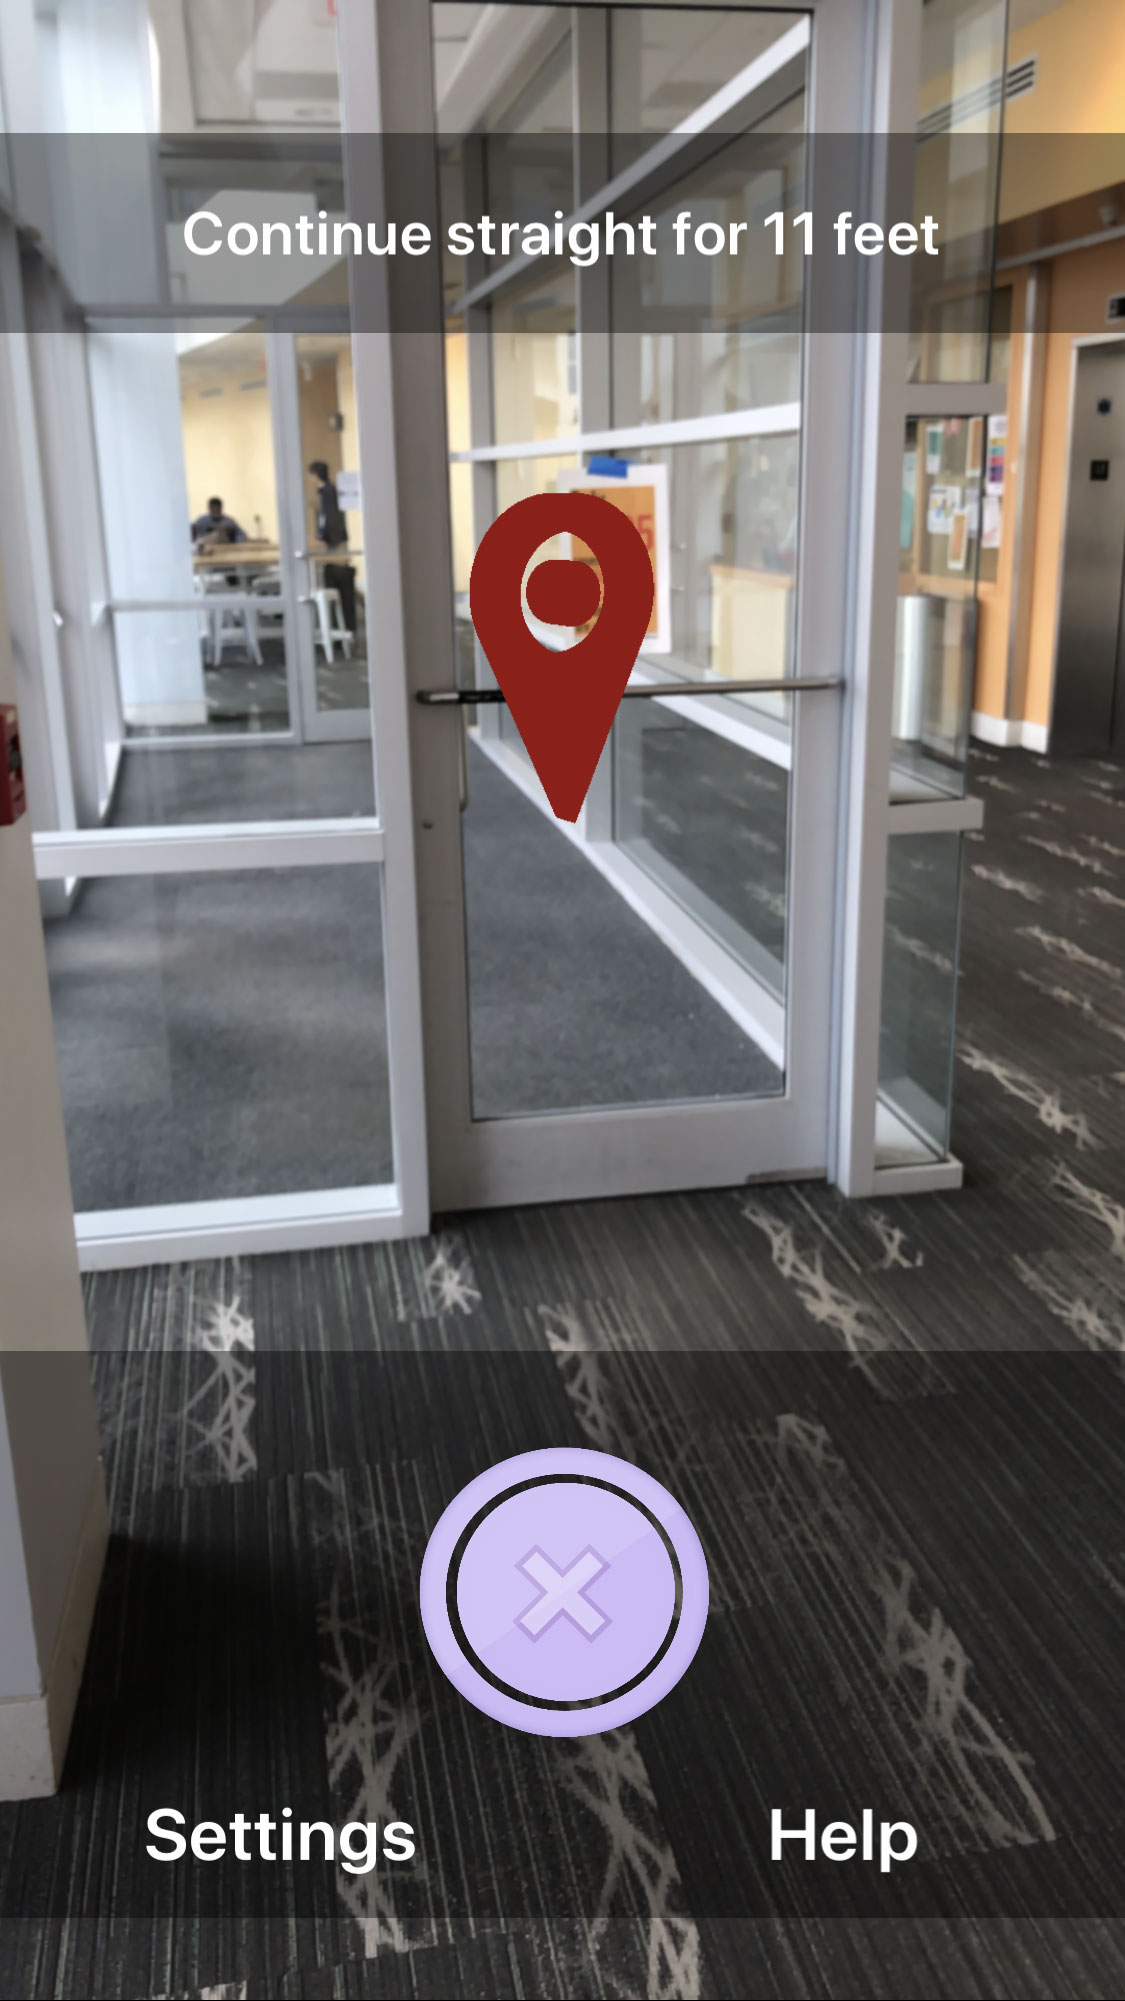
\includegraphics[width=0.42\linewidth]{Figures/clew_screenshot_15}\hspace{.01\linewidth}
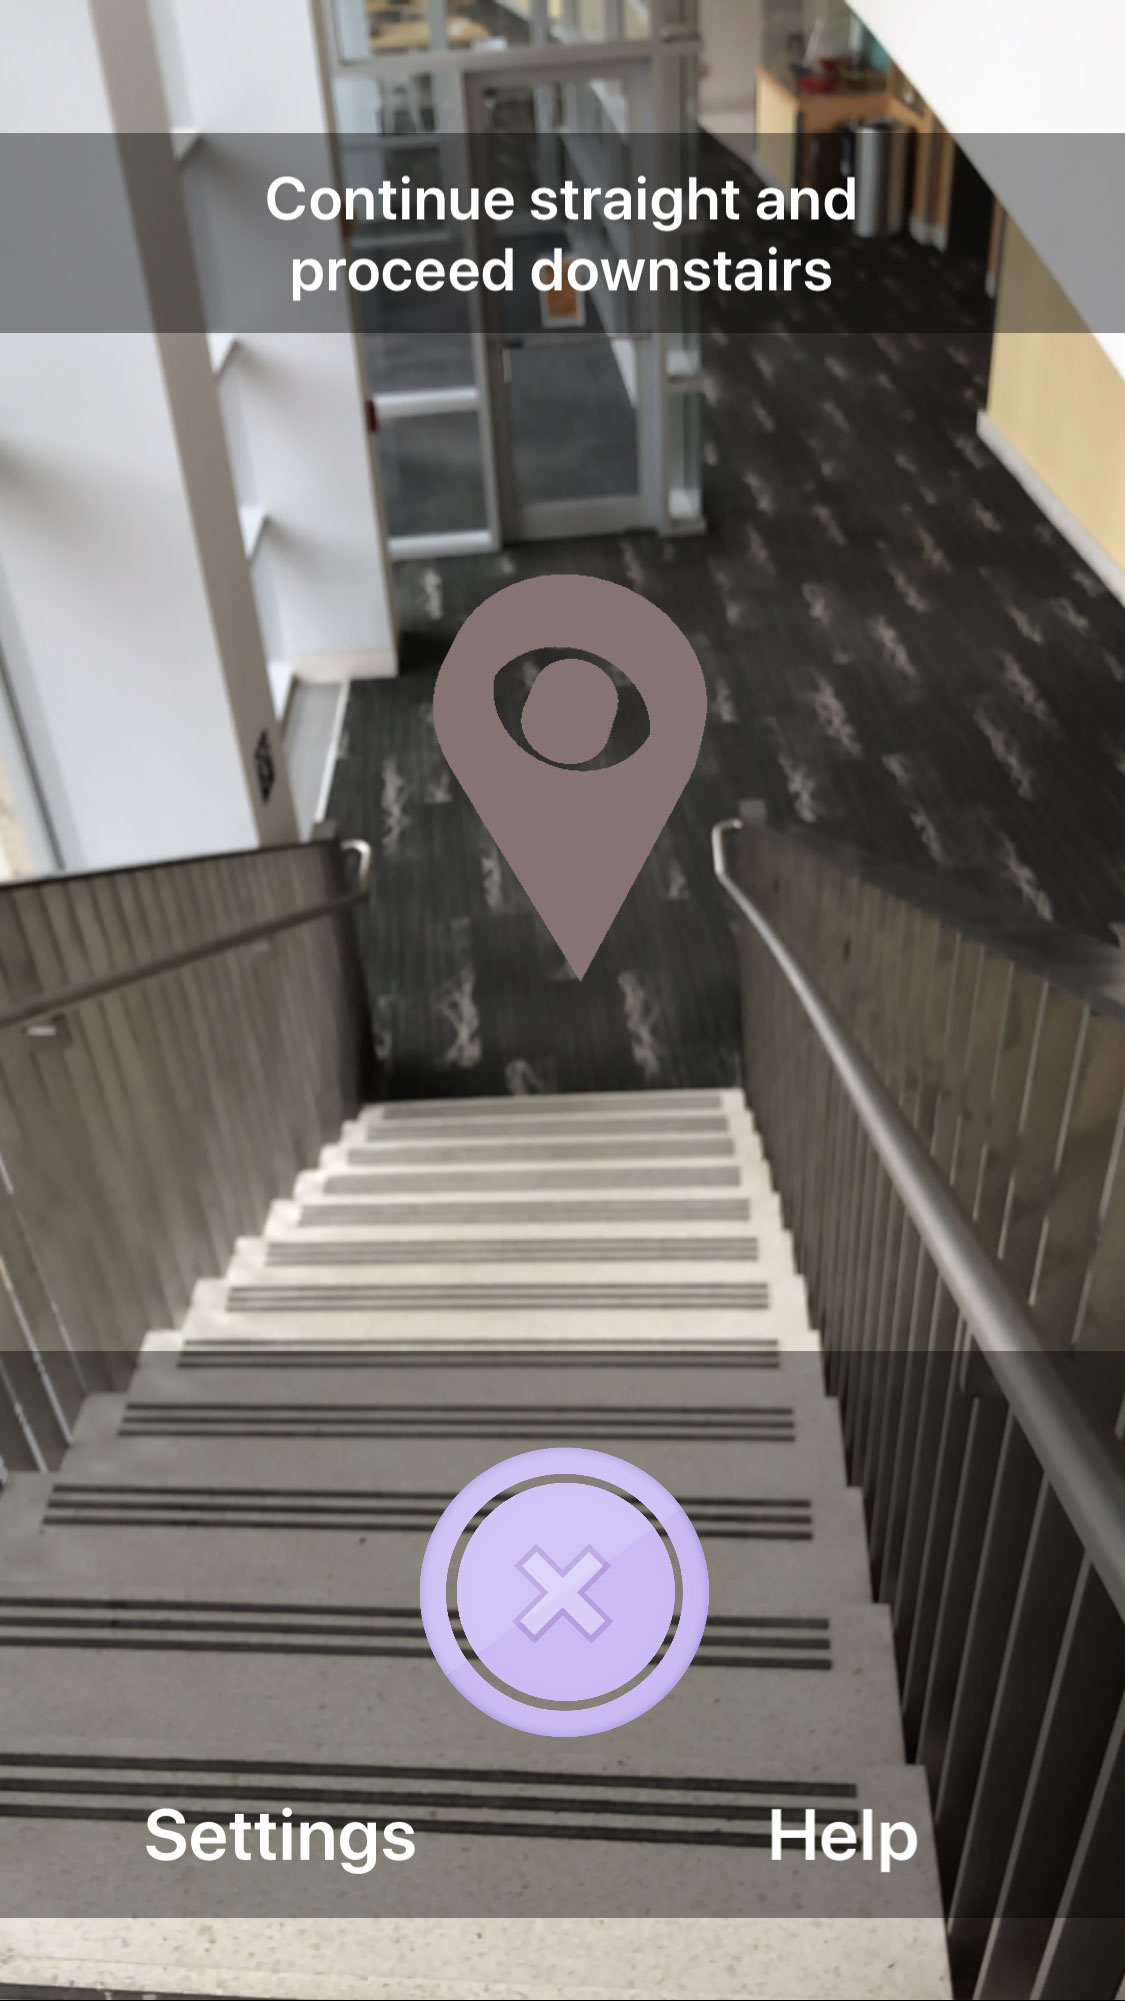
\includegraphics[width=0.42\linewidth]{Figures/clew_screenshot_6}
\end{center}
\caption{Two screenshots from the app ``Clew.''  The text for the left image says ``Continue straight for 11 feet'' and the text on the right says ``Continue straight and proceed downstairs.''\label{fig:clewshots}}
\end{figure}

\begin{figure*}
\begin{center}
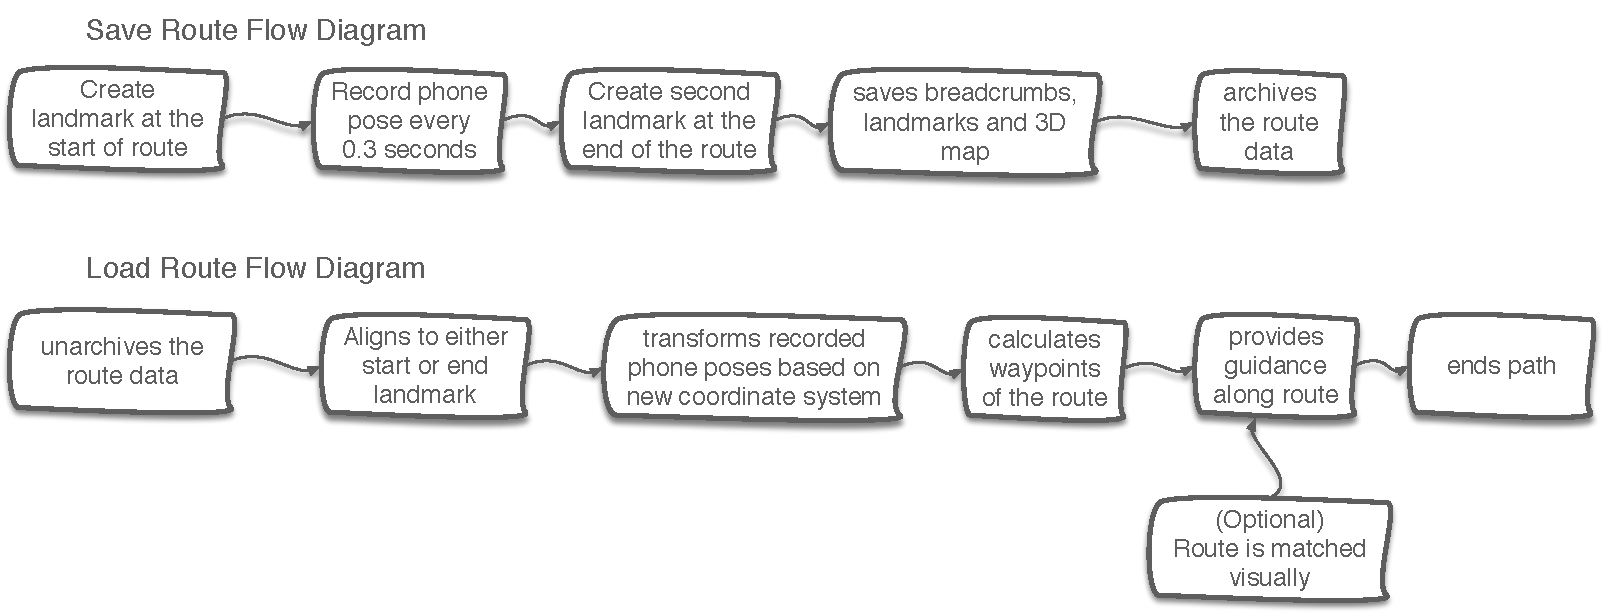
\includegraphics[width=.7\linewidth]{Figures/FlowDiagram}
\end{center}
\caption{A flow diagram of the process for both saving and loading routes in \emph{Clew}.\label{fig:flow}}
\end{figure*}

\subsubsection{Registration through Visual Alignment}
With the release of iOS 12.0, Apple's ARKit supports a re-localization feature whereby a visual representation of landmarks and their associated 3D positions form a sparse map of an ARKit session.  Given a new ARKit session (e.g., the user has restarted the app), ARKit can load the previous 3D map and attempt to match the phone's current image features to the map.  If a match is found, the current position and orientation of the phone are updated to be relative to the coordinate system in the 3D map (thereby registering the two coordinate systems).  In order to support route saving and pausing, \emph{Clew} saves the current 3D map of the tracking session and attempts to use visual alignment to relocalize the user.% when the user wants to reload the route.

The main limitation of visual alignment is that it doesn't always succeed.  This can occur for a multitude of reasons.  First, if the environment has changed significantly, for instance when lighting conditions have changed drastically, the visual environment may not look similar enough to the saved 3D map.  Alternatively, even if the environment is static, the user's viewing angle might be significantly different.  This is particularly likely to happen when navigating routes in the reverse direction as visual features in the environment often appear very different when viewed from the opposite direction.  Anecdotally, ARKit's visual alignment feature appears to be tuned conservatively.  That is, when a match is found it is almost always a correct match.


\subsubsection{Registration through Physical Alignment}

In order to allow users to reload or pause routes when visual alignment is impossible, Clew supports physical alignment through landmarks.  A user can create a landmark by placing their phone in a position and orientation (collectively called a ``pose'') that is easy to return to, unassisted, when the user wants to resume or reload the route.  The most important aspect of the pose that the user must successfully recreate is its yaw.  The reason for this is that the phone's accelerometer can determine pitch and roll, which are not perpendicular to gravity, and deviations in the phone's position contribute a fixed amount of error, whereas an error in the phone's yaw will be magnified over long routes.

The procedure for landmark creation is for the user to place their phone's top (short-edge) flush against a flat vertical surface (such as a door or wall).  In this configuration, the user's camera will be facing down, which will allow it to track visual features on the floor, and the screen will be facing up, which allows the user to see what's on the screen (if they have usable vision) or interact with the phone using VoiceOver.  In order to make the alignment process more robust, we artificially ``level'' the phone by undoing the effects of roll and pitch to create a virtual landmark pose in which the phone is perfectly flat.  Anecdotally, we found that this leveling process was important for maximizing accuracy.  Clew allows the user to enter text or record a voice message to help them remember how they positioned their phone when creating the landmark (e.g., ``Office front door, right above the handle'').  While in theory we could support registration with visual alignment only, we made the design decision to require the user to physically register a landmark in order to reload or pause a route.  A diagram of the route saving and loading procedures is shown in Figure~\ref{fig:flow}.

\subsection{Path Navigation Mode}\label{sec:pathnavigationmode}

When the user is ready to navigate a route, the trail of breadcrumbs is processed by the Ramer-Douglas-Peucker (RDP) algorithm \cite{douglas1973algorithms} for path simplification.  This algorithm winnows down the path by removing sequences of breadcrumbs that are well represented by a straight line.  Figure~\ref{fig:samplepath} shows the breadcrumbs selected by the RDP algorithm, called \emph{waypoints}, and the resultant piecewise straight navigation route obtained by connecting the waypoints.  In \emph{navigation mode}, the app synthesizes directions to the next waypoint using one of three mechanisms: (1) speech (e.g., ``continue straight for 10 feet''), (2) haptic or (3) audible feedback when the phone is pointing towards the next waypoint.  When using (2) or (3), the low latency of the update of the phone's position allows the user to sweep their phone back and forth until they sense a haptic or auditory cue, providing an accurate sense of the direction to the next waypoint.

As the user navigates, the app continuously checks to see if the user has reached the next waypoint.  We define the condition of ``reached the next waypoint'' as the user entering a \emph{waypoint checkoff zone} (see Figure~\ref{fig:samplepath}).  Instead of using spherical checkoff zones, we use rectangular prisms whose sides which are perpendicular to the direction of travel are longer than for those that are parallel to the direction of travel.  This choice of shape enables the user to deviate laterally from the intended path without missing a waypoint.  The app also announces flights of stairs by detecting if the vertical angle of the segment connecting two waypoints exceeds a threshold.

\section{Usability Testing and Technology Evaluation}\label{sec:usabilityandevaluation}
Here, we discuss the results of co-designs as well as data analyses that informed the creation of specific aspects of Clew. % A number of our results have implications for researchers who would like to use AR technology to create assistive apps for people who are \BVI.

\subsection{Longitudinal Design with Local Co-Design Partners}
As discussed in \emph{Design Process Overview}, we engaged with each of our four co-designer partners for five, three-hour sessions at a frequency of one visit per week.  The first co-design partner, Joe, worked with us during the summer of 2017 and was instrumental in developing the initial concept of Clew.  The other three co-designers (pseudonyms Carmen, Karen, and George) worked with us during the summer of 2018 and contributed useful insights along a range of dimensions.  Here we highlight several of these insights that are of particular relevance to using AR technology for people who are \BVI.

\subsubsection{Insight 1: Maintaining Optimal Phone Orientation}
VIO algorithms work best when they detect visual features at a range of depths from the camera.  The reason for this is that many of these algorithms perform geometrical calculations which are best numerically conditioned in such situations.  This suggests that users should hold their phone upright with the camera facing approximately parallel to the ground.  If the user's phone is pointed down at the floor or to the side at a wall, the phone will track features that primarily lie on a single plane, which will result in less reliable estimates of motion.  Both Joe and George had difficulty maintaining their phones in this configuration (perhaps due to the lack of visual feedback about the phone's orientation).  As a result, tracking performance suffered.  In our large-scale evaluation, we were able to demonstrate this quantitatively.  Developers of AR-powered assistive apps may consider adding feedback mechanisms to help the user to maintain their phone in a vertical, forward-facing orientation.

\subsubsection{Insight 2: Alignment Between Body and Phone}
Through our interactions with George we discovered that some users have a difficult time understanding the orientation of their phone relative to the orientation of their body.  George is congenitally blind, whereas the other three co-designers, none of whom had this difficulty, lost their vision in their teens.  That the age at which sight was lost would have this effect was not wholly unexpected (see, e.g., \cite{long1997establishing, wiener2010foundations, schinazi2016spatial, thinus1997representation, williams2014just} for discussions of how spatial processing differs based on when the onset of vision loss occurred).  While George could easily rotate his body in an effort to elicit haptic guidance from the app, which would indicate that the phone was facing the correct direction, he was not able to rotate the phone in his hand (with his body stationary), sense that the phone was pointing in the correct direction, and then align his body with the phone's direction.

Even if George scanned for the next waypoint by rotating his body, a second difficulty presented itself.  George had difficulty keeping the phone pointing straight ahead.  Instead, the phone would often point to the side at an angle of greater than 30 degrees.  Since this angular offset would make the app's directions inaccurate, we developed a method to provide feedback relative to the user's body direction rather than the phone's direction.  The method works by constantly updating an estimate of the phone's offset relative to the user's body.  The calculation of this offset is performed when the user is moving forward (moving laterally will throw this calculation off).  We found that this modification enabled George to use the app.  Researchers should be cognizant of the differing abilities of users to sense spatial relationships between various parts of their body and their phone.

\subsection{Quantitative Evaluation of ARKit's Accuracy}

\begin{table}
  \centering
  \begin{tabular}{c c c}
    % \toprule
    {\small \textit{Route Length}}
      & {\small \textit{Contains Staircase}}
        & {\small \textit{Mean Error}}  \\
    \midrule
    10m & yes  & 0.27m \\
    13m & no & 0.51m \\
    26m & yes & 0.74m \\
    38m & no & 0.56m \\
        63m & yes & 0.50m \\
    % \bottomrule
  \end{tabular}
  \caption{Accuracy of relative position estimates for the start and end of the route.  This number is indicative of the navigation accuracy that could be expected when using Clew over a similar route.\label{tab:clewaccuracy}}%  The \emph{Visuals} column indicates the availability of trackable visual features, with ``mixed'' indicating that a route had segments of both high and low availability.}~
\end{table}

In order to better understand the accuracy of ARKit for navigation, we performed a benchmarking experiment to test ARKit's performance along five indoor routes of varying length and complexity.  For each route, the phone was placed flush against a wall in a particular starting location.  Once the phone was positioned properly, the \emph{landmark procedure} (described earlier) was performed.  Next, the experimenter walked the route (using their vision) to the route's endpoint where the landmark procedure was  performed a second time.  The relative position of the ending landmark to the beginning landmark provided an estimate of the spatial relationship between these two points.

To get a sense of how repeatable the estimate of the spatial relationship between the start and end of the route was, we repeated this process at least seven times per route (longer routes were repeated more times to smooth out the larger variability of errors for these routes).  The error associated with both the physical alignment procedure (landmark creation) as well as the drift incurred by ARKit while navigating the route was quantified by calculating the mean distance between the centroid of the estimated relative positions between the landmarks and the relative position computed on a particular trial.  This metric provides a sense of how accurately ARKit could give feedback to the user regarding how close they are to the route's endpoint.  While it does not say anything about the accuracy of ARKit in the middle of the route, the endpoint is likely to be where the error is greatest (as it is the farthest from the start and thus more motion tracking error has accumulated).

The characteristics of the routes tested as well as the accuracy of the relative start-to-end position estimates are shown in Table~\ref{tab:clewaccuracy}.  Even over routes as long as 63m, the error is under 1 meter.  This holds true  when the route involves ascending or descending stairs.  These results support the idea that ARKit's tracking performance is accurate enough for use in guiding users along recorded indoor routes of moderate length.

\subsection{Feedback from Global User Community}
In order to achieve impact on a large-scale and to understand the performance of our app at a fine-grained, quantitative level, we released \emph{Clew} on the iOS app store in 156 countries.  In this section, we summarize the most important lessons we learned from the global community as to how to utilize AR technology to create assistive technology for people who are \BVI.

\subsubsection{Adoption and Usage of Clew}

We initially promoted the app on a limited basis through word-of-mouth to local members of the \BVI community.  Several members of the community discovered Clew and created posts on the popular assistive technology portal \emph{Applevis}.  The publicity created by the \emph{Applevis} posts generated a number of additional articles, podcasts, and blog entries.  As of the publication of this paper, Clew has been downloaded by over 5,000 people from 50 different countries.  Clew is used by an average of 60 people per day.

\subsubsection{Selected Feedback from the Community}
We received dozens of e-mails from users providing feedback on Clew.  While feedback of this form does not constitute a scientific, randomized sampling of sentiment from Clew's user base, it does provide actual stories that validate that Clew is useful to real people.  Here is a sampling of quotes from the e-mails we received that provide evidence along these lines.

\begin{itemize}
\item ``I find it incredibly accurate when it comes to backtracking and navigating in places that may or may not be very complicated to get around as someone who is blind or visually impaired.''
\item ``I used the app to navigate from the garage back to my bedroom, and it totally helped me in giving me clear instructions with VoiceOver running and the sounds that tells me where to turn next.''
\item ``I've tested the new version of your app.  I Am very happy and impressed by the this latest version!  Especially the “save routes” feature makes it a very useful app \ldots I think the app will be a great help for recording routes in train stations, big shops etc.''
\item ``First, I should admit that this is really an innovative idea to
use in-door navigation. I tried the app many times and it works like a
charm in all trials.''
\item ``I am so satisfied from this application.  I use it in my daily life.''
\end{itemize}


\subsubsection{Designing for Low-Vision Users}
One somewhat surprising thing we heard from the community is that Clew was useful for people who are low-vision (rather than just people who are blind).  In our design of the initial version of Clew, we had focused on making Clew  accessible via VoiceOver.  We didn't put much intentionality into the visual design of the app for people with low vision.  When the app began to gain popularity we received feedback that the app's text was too small, the visual design of the waypoint markers was suboptimal, and that our speech guidance did not work if VoiceOver was turned off.  We addressed many of these concerns in subsequent updates.

\subsubsection{Supporting Older iOS versions}

In response to a beta version of the app that removed support for an older version of iOS, one user expressed a desire to maintain this support.  We were puzzled by this request as we assumed that all users would have upgraded to the most recent iOS (which was 12.2).  The user explained that he didn't update his phone until the new major revision had been out for a significant amount of time.  He went on to say that the minor bugs that often accompany major releases that sighted users can workaround can be showstoppers for people that rely on the accessibility features of iOS.  As a result, we reversed course and maintained support for older iOS versions.

\subsubsection{Importance of Internationalization and Localization}

The majority of the users of Clew are from outside of the U.S.  The fact that Clew was released, and is still available only in English, is a limiting factor in the adoption and successful usage of Clew.  We have received many requests for Clew to be localized into other languages as well as a number of offers to perform localization work pro bono.  If we think of the users of the app as co-designers first and foremost, by not localizing the app, we are missing out on a lot of potential insights. %  The fact that language barriers created a lack of accessibility for an app designed to promote indoor accessibility was an irony we had not thought about ahead of time.

\subsection{Large-Scale User Study}\label{sec:largescalestudy}
\begin{figure}
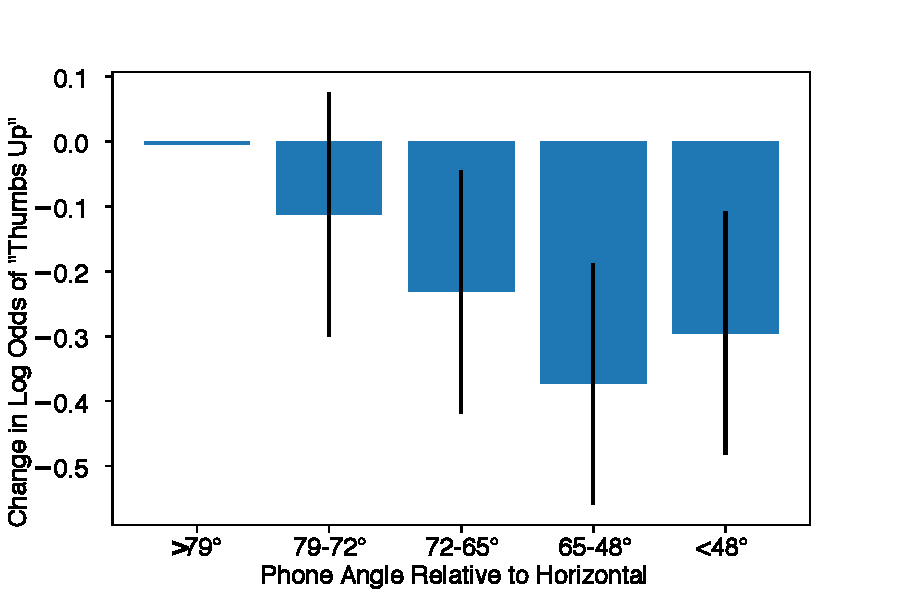
\includegraphics[width=\linewidth]{figures/phoneangle}
\caption{The relationship between log odds of the user rating a navigation experience as ``thumbs up'' and the median angle of the phone relative to horizontal (i.e., a plane perpendicular to gravity).  Also shown are the 95\% confidence intervals.\label{fig:devicepose}}
\end{figure}

After the user successfully completes the navigation of a route or cancels navigation, they are prompted to rate the quality of the app's navigational guidance as either ``thumbs up'' or ``thumbs down.''   While the exact meaning of these ratings is subjective (we don't provide any guidance to the user about what these mean), it does provide us with data to understand the factors that influence the quality of the user's experience.  Importantly, users could opt out of contributing their route ratings and log data, so we only have access to data that represents a subset of the overall usage of the app.

In order to investigate the association between various factors and the user's rating of a navigation experience, we performed a logistic regression analysis with route rating as the dependent variable and the following independent variables.
\begin{itemize}
\item a binary feature that indicated whether or not the route was resumed/reloaded versus newly recorded
\item a binary feature that indicated whether the route was in the same direction of the recording or in the reverse direction
\item a categorical feature that indicated which of five percentile bins the length of the route fell within (0-20th percentile, 20th-40th percentile, 40th-60th percentile, 60th-80th percentile, 80th-100th percentile).
\item a categorical feature that indicated the number of motion tracking errors reported by ARKit during the route navigation (0, 1, 2, 3, or more than 4).
\item a categorical feature that indicated the median angle of the user's device relative to the ground plane during route navigation.  The feature indicated which of five percentile bins the median device angle fell within (0-20th percentile, 20th-40th percentile, 40th-60th percentile, 60th-80th percentile, 80th-100th percentile).
\end{itemize}

In total, our analysis covered 5,789 routes.  A total of 490 of these routes were collected after we released support for route saving and reloading (in the first few versions of Clew, route pausing was supported but not route reloading).  The baseline ``thumbs up'' rating in the dataset was 68\%. 

\subsubsection{Importance of Device Pose During Navigation}


As mentioned previously, we knew from both the underlying details of the algorithms and from our anecdotal observations that VIO performed sub-optimally when the phone was not held vertically.  Further, we had seen that some of our co-designers had difficulty keeping the phone vertical while using the app. The regression analysis showed that, consistent with these observations, users were less likely to rate their navigation experiences positively when the phone was held at a flatter angle.  Figure~\ref{fig:devicepose} shows the coefficients of our logistic regression analysis.  Once past the 72 degree threshold, the categorical values have confidence intervals that do not overlap with 0 (implying a statistically significant reduction in likelihood of a positive rating at these flatter angles) but do overlap with each other (implying that no statistically significant difference was found between categorical values past 72 degrees).  This finding further underscores the utility of providing feedback to help the user maintain their phone's vertical orientation.

\subsubsection{Importance of Minimizing Tracking Failures}
\begin{figure}
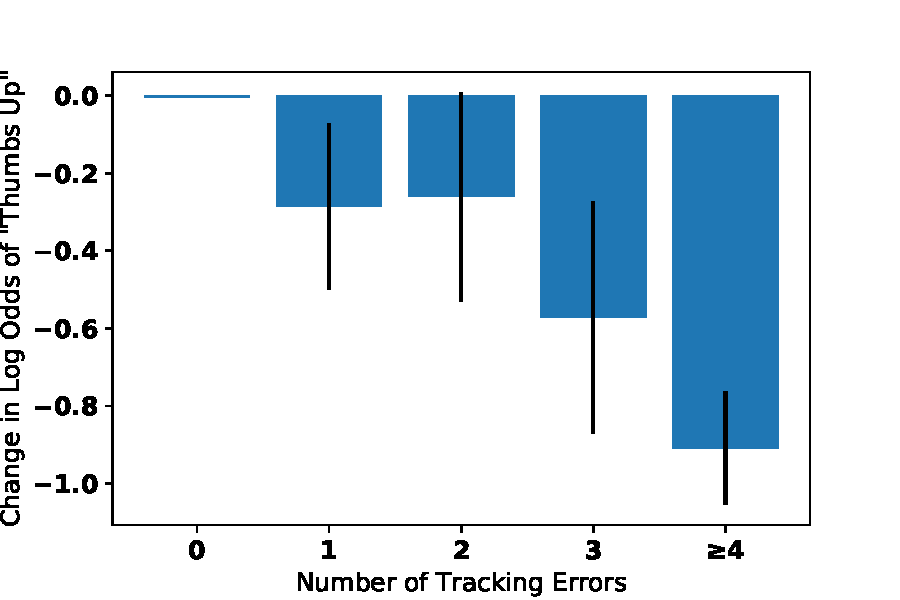
\includegraphics[width=\linewidth]{figures/trackingerrors}
\caption{The relationship between log odds of the user rating a navigation experience as ``thumbs up'' and the number of tracking errors encountered during route navigation.  Also shown are the 95\% confidence intervals.\label{fig:trackingerrors}}
\end{figure}

ARKit reports two error conditions related to motion tracking.  One error condition is ``insufficient visual features,'' which occurs when the camera is not capturing images with sufficient texture to allow for accurate feature tracking.  The second error condition is ``excessive motion,'' which occurs when the phone is moving too quickly.  Our analysis found that there was a steep drop-off in the likelihood of the user rating the navigation experience positively as the number of tracking errors increased (see Figure~\ref{fig:trackingerrors}).  This finding prompted us to change the behavior of the app to announce tracking errors to the user in hopes that this feedback would help the user to avoid them.

\subsubsection{Route Characteristics and Average Rating}
In addition to the quality of the tracking of the user's phone during navigation, we also found that various characteristics of the route itself were related to the likelihood of the user providing a positive rating to their navigation experience.

\begin{figure}
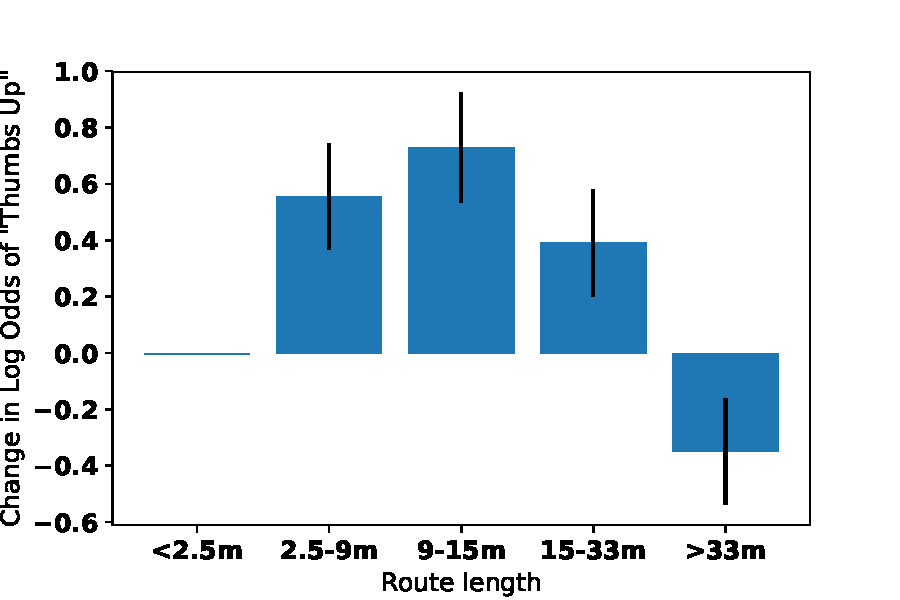
\includegraphics[width=\linewidth]{figures/routelength}
\caption{The relationship between log odds of the user rating a navigation experience as ``thumbs up'' and the length of the route.  Also shown are the 95\% confidence intervals.\label{fig:routelength}}
\end{figure}

\begin{table}
  \centering
\begin{tabular}{c  c c c c c c}
{\small \textit{feature}}	& {\small \textit{coef}}  & {\small \textit{p-value}} & {\small \textit{95\% confidence interval}} \\
intercept	& 1.3731&	0.000 &	[0.850 ,1.897] \\
%C(navigationVerticalityMedianQCut)(-0.981, -0.954] &	-0.1133	& 0.096 & 	-1.181&	0.238 &	-0.301& 0.075 \\
%C(navigationVerticalityMedianQCut)(-0.954, -0.908] &	-0.2319	& 0.095 &	-2.435	&0.015 &	-0.419	& -0.045
%C(navigationVerticalityMedianQCut)[T.Interval(-0.908, -0.748, closed='right')]	-0.3733	0.095	-3.945	0.000	-0.559	-0.188
%C(navigationVerticalityMedianQCut)[T.Interval(-0.748, 0.993, closed='right')]	-0.2953	0.095	-3.093	0.002	-0.482	-0.108
%C(numTrackingErrorsLimited)[T.1.0]	-0.2849	0.109	-2.614	0.009	-0.499	-0.071
%C(numTrackingErrorsLimited)[T.2.0]	-0.2608	0.137	-1.901	0.057	-0.530	0.008
%C(numTrackingErrorsLimited)[T.3.0]	-0.5718	0.153	-3.747	0.000	-0.871	-0.273
%C(numTrackingErrorsLimited)[T.4.0]	-0.9092	0.074	-12.280	0.000	-1.054	-0.764
%C(routeDistanceQCut)[T.Interval(2.634, 9.37, closed='right')]	0.5567	0.096	5.786	0.000	0.368	0.745
%C(routeDistanceQCut)[T.Interval(9.37, 15.486, closed='right')]	0.7283	0.100	7.302	0.000	0.533	0.924
%C(routeDistanceQCut)[T.Interval(15.486, 32.801, closed='right')]	0.3905	0.097	4.022	0.000	0.200	0.581
%C(routeDistanceQCut)[T.Interval(32.801, 453788.499, closed='right')]	-0.3496	0.096	-3.656	0.000	-0.537	-0.162
is resumed route?	& -0.5189	& 0.002 & [	-0.840 ,	-0.198 ]\\
is end to start?	& -0.3331	& 0.182	& [-0.822, 0.156]
\end{tabular}
  \caption{Logistic regression analysis for the two binary features and the intercept term.\label{tab:binaryfeatures}}
\end{table}

Routes that were resumed (versus newly recorded) had a lower log-likelihood ratio of being rated positively ($p < 0.002$).  This finding is consistent with the inaccuracies that can be introduced by Clew's route alignment procedure.  Routes that were resumed but navigated in the forward direction had a higher likelihood of being rated positively, but the result was not statistically significant ($p = 0.2$). If this finding holds, this is likely related to the higher success rate of visual alignment when navigating in the forward direction where visual features are more similar to those seen during route recording.  These findings are summarized in Table~\ref{tab:binaryfeatures}.


The relationship between route length and the likelihood of a positive rating had an unexpected form (see Figure~\ref{fig:routelength}).  The figure shows that the navigation experiences that are most likely to be rated positively are for routes that are between 9 and 15 meters in length. We had expected that the likelihood of a positive rating would monotonically decrease with route length.  We think this is due to the fact that users are forced to rate every route and have no way to cancel navigation without issuing a rating.  The lower ratings for shorter routes could be due to users wanting to cancel route recording and being forced to issue a rating of a route they didn't intend to record.

\section{Summary of Considerations for Researchers who Want to Use Smartphone-based AR for \OM}

Based on our co-design process, technology evaluation, and user study, we summarize our advice for assistive technology researchers who want to use AR for \OM as follows.

\begin{itemize}
\item \emph{Without any additional environmental instrumentation, ARKit is robust enough for many indoor navigation scenarios}.  Our study demonstrates that for navigation routes of $\sim61m$ the motion estimates of ARKit are accurate.
\item \emph{There is a discrepancy between the accuracy of ARKit (as determined in our internal tests) and the fact that routes longer than $33m$ are unlikely to be rated positively}.  Our hypothesis is that this is due to usability concerns of both our app specifically and AR technology more generally.

\item \emph{Maintaining the phone in a vertical orientation is important for optimal performance}.  It is an open question as to how to incorporate this finding into the design of the user experience of an app (e.g., whether it is a good idea to provide explicit feedback when the phone is too flat).
\item \emph{Design for multiple levels of vision}.  While it is tempting to think of apps in this space as special-purpose assistive technology, based on our experience we feel that taking a universal design approach will make the end product useful to people who you didn't imagine were part of your user group (e.g., users who are low-vision).
\item \emph{Consider differing abilities to process spatial information}.  In addition to the spectrum of visual abilities of users, users will have a spectrum of ability to understand spatial relationships between various parts of their body and their phone.  Providing mechanisms to alleviate the need for the user to have a highly precise sense of space will make an app more widely usable.
\item \emph{Consider investing in internationalization and localization upfront}.  Since blindness is a low-incidence impairment, to get a broad sample of users may require working with people on a global scale.  Releasing an English-only app sends a message of exclusion to would-be co-designers.

\item \emph{Design your interface with distributed co-design in mind}.  The feedback mechanism of ``thumbs up'' versus ``thumbs down,'' provides a relatively narrow lens to understand the user experience using the app.  Consider building in a richer set of feedback mechanisms to gather information from users about how your AR-powered app is functioning for them in their particular environment.  Thinking of those that use your app as co-designers, rather than testers, may help in framing how you think of these interfaces.


\end{itemize}


%\section{App 2: ViewShare}
%
%Finding objects in unfamiliar environments can be challenging for people who are \BVI.  Inspired by previous work \cite{bigham2010vizwizlocateit} that utilizes a crowdsourcing model, whereby sighted online volunteers label an object of interest and sonic cues automatically guide a user to an object, we developed the \emph{ViewShare} app.
%
%\emph{ViewShare} provides high precision, automatic guidance to objects of interest.  To begin, the user, who is \BVI, launches the ViewShare app, starting an ARKit tracking session.  When the user wants to find an object, they announce its name, the phone recognizes their voice command, and a localization job is created.  This job is assigned to multiple sighted volunteers, who are sent push notifications on their smartphones.  On the \BVI user's device, every two seconds a snapshot of their environment is captured and added to the job.  Once a volunteer clicks on the push notification they are shown the snapshots (see Figure~\ref{fig:viewsharescreenshots}).  After the volunteer locates the object, they tap its position on the screen.  The object location in the image, represented as a 2D pixel coordinate, is relayed back to the \BVI user's app, which then attempts to convert this coordinate into a 3D position (see \emph{2D to 3D Transformation}).  If a 3D location can be determined, the user is provided with automatic guidance to the object in the form of computer-generated speech and haptic feedback.
%
%\subsection{Object Localization Feedback}
%ViewShare communicates location information using haptic and speech feedback.  Specifically, whenever the phone is oriented towards a located object the phone will vibrate subtly and the distance and name of the object will be announced.  To facilitate finding objects in 3D, the app provides two localization modes.  In \emph{2D feedback mode} the distance and orientation to an object are determined by projecting 3D spatial information into the floor plane.  This mode is useful for navigating to objects that are far away (since the height of the object is irrelevant until the user gets closer).  In \emph{3D feedback mode} distances and orientations to objects are determined using the unmodified 3D information.  This mode is useful for finding objects that are nearby.%  As an example, 3D mode is suited to finding a pen and 2D mode is suited to finding a door.
%
%\begin{figure}
%\begin{center}
%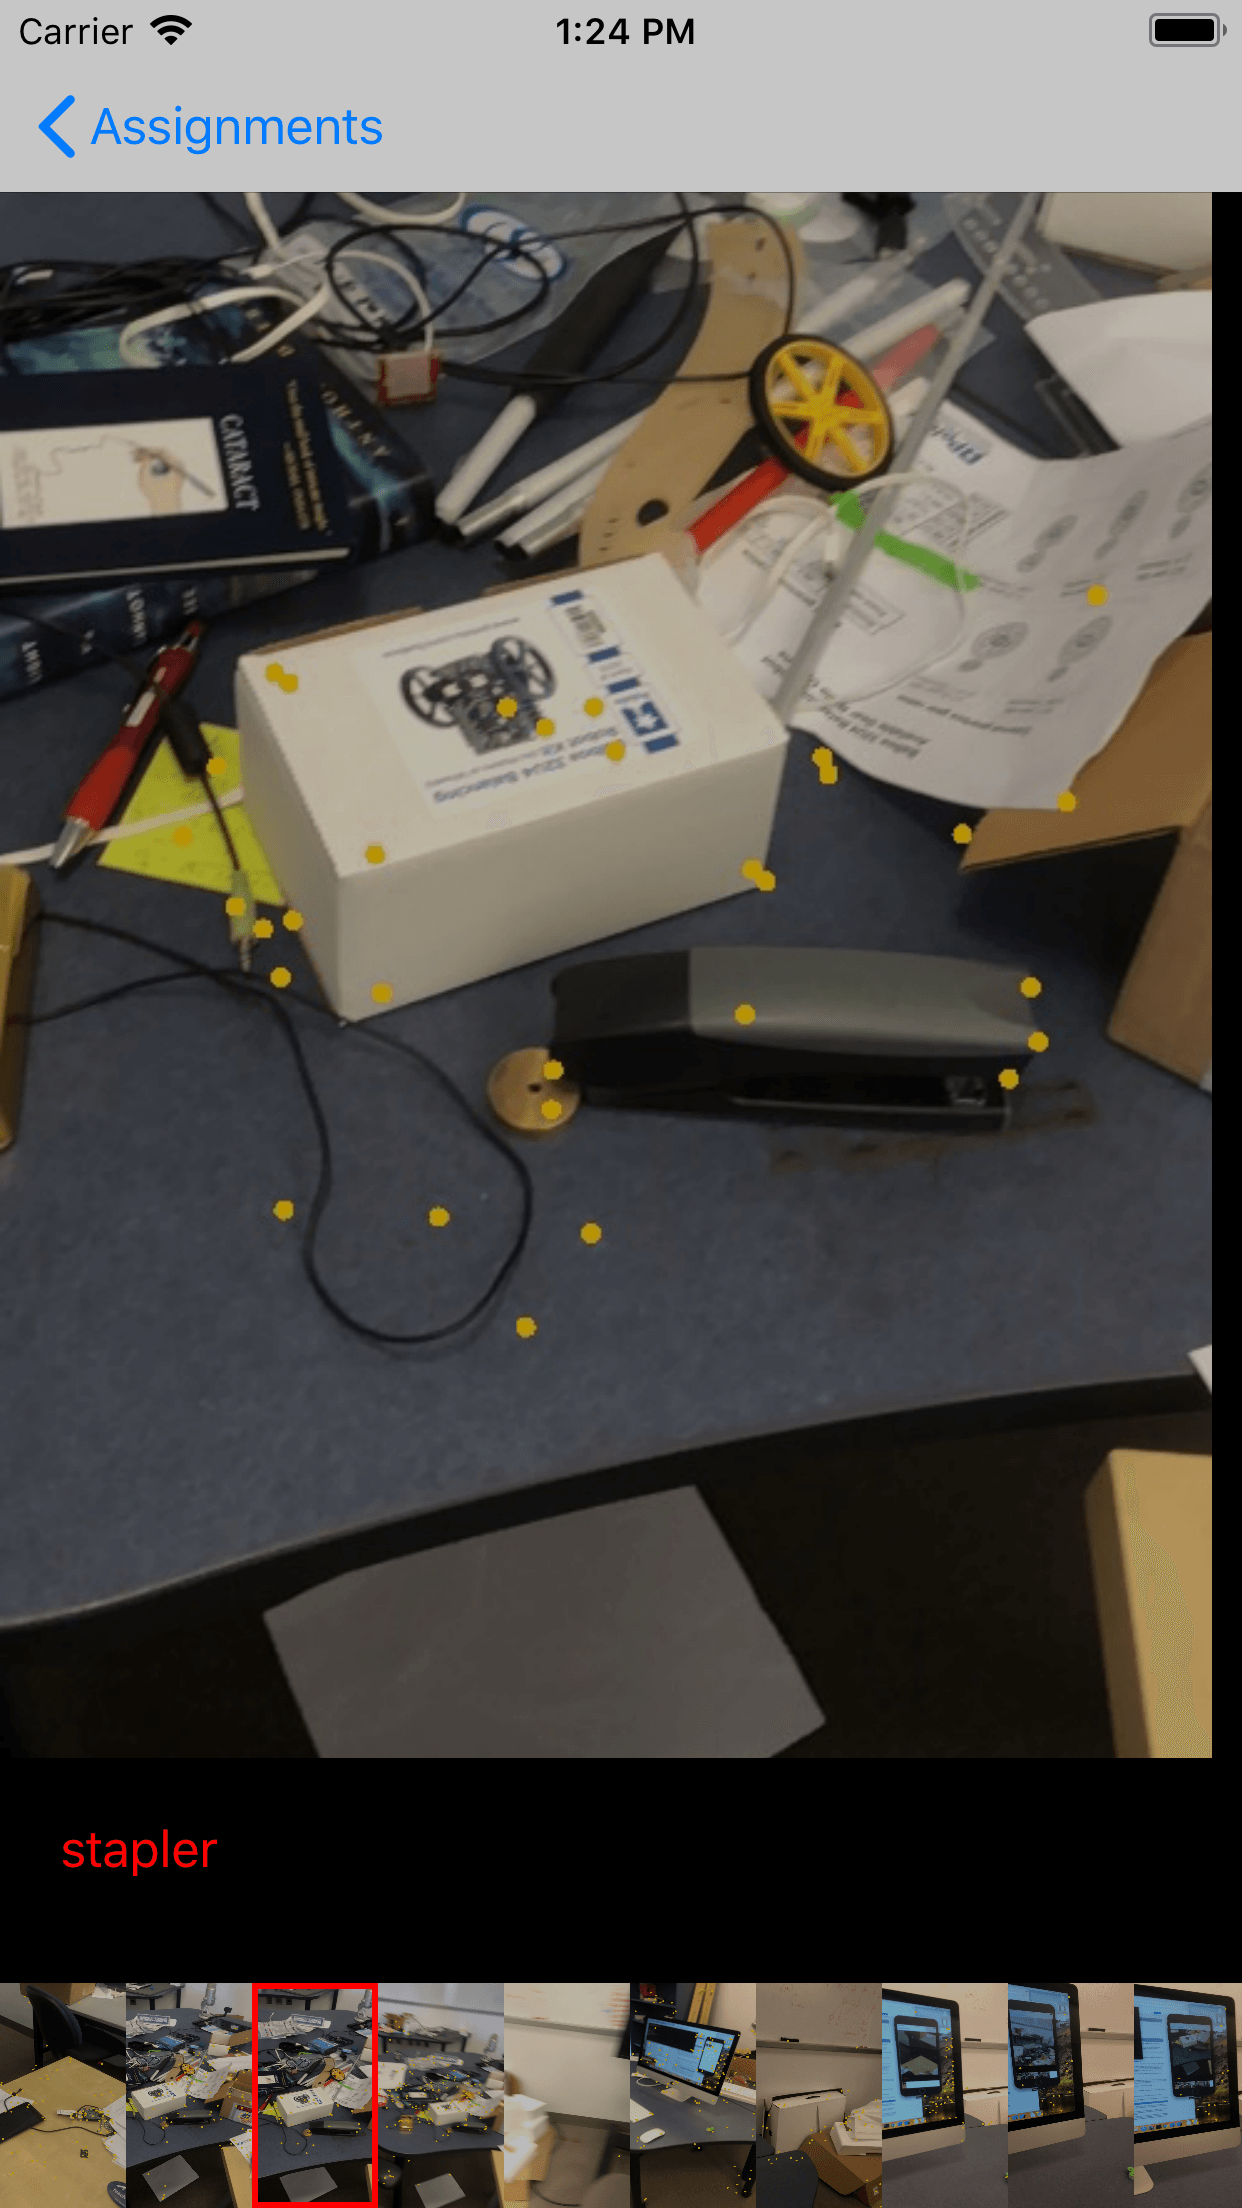
\includegraphics[height=3in]{Figures/viewshare_crowdworker}\hspace{.01\linewidth}
%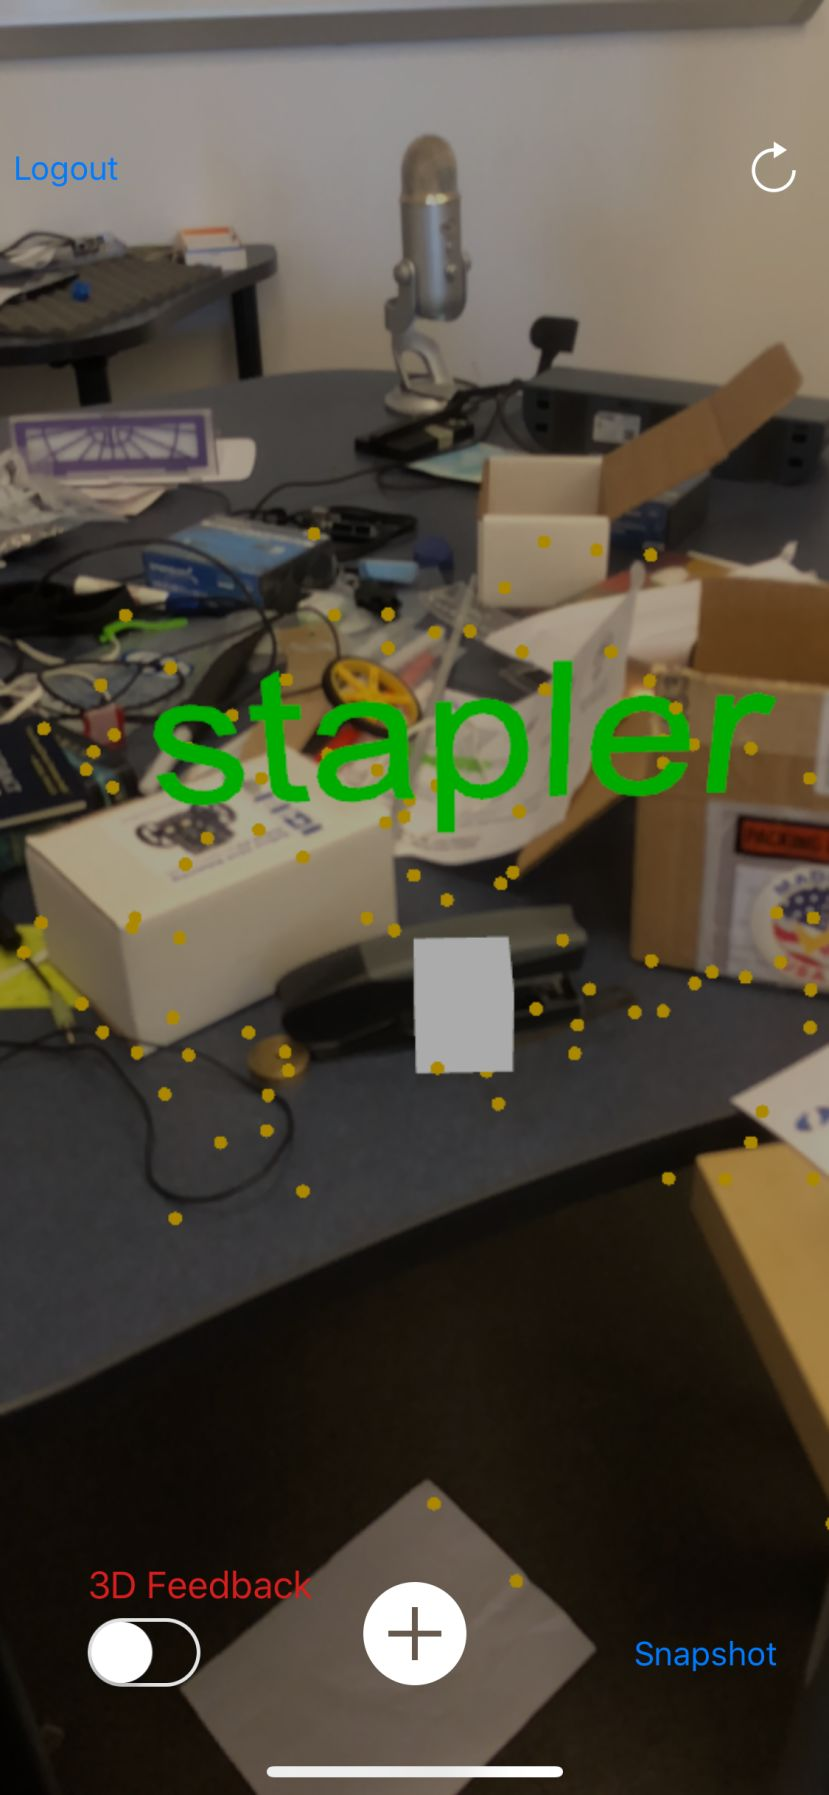
\includegraphics[height=3in]{Figures/viewshare_user}
%\end{center}
%\caption{Left: ViewShare's interface for the crowdworker.  The crowdworker is instructed to locate the stapler in the images collected from the \BVI user's phone.  \textbf{Right:} the interface for the \BVI user showing the location of the stapler as indicated by the crowdworker (the visualization is useful primarily for users with low vision and as a debugging tool).\label{fig:viewsharescreenshots}}
%\end{figure}
%
%
%\subsection{2D to 3D Transformation}
%In order to map a 2D pixel coordinate to a 3D point in space, we utilize ARKit's plane fitting feature.  We first test whether the ray that connects the optical center of the camera with the location of the pixel coordinate of the located object intersects a tracked 3D plane (ARKit is capable of finding both vertical and horizontal planes in 3D).  If the ray intersects a plane, we mark the object as localized and compute its 3D position using standard geometric formulas.  If the ray \emph{does not} intersect a known plane (either because the object is not located on a plane or because the plane has not been found by ARKit) we return an error condition.  In this situation, the volunteer is instructed to click on the object from a second viewpoint.  Once the 2D pixel coordinate of the object is provided in two views, we use triangulation to compute its 3D position. % The optimal 3D triangulation of two rays with endpoints $x_1$ and $x_2$ and unit directions $u_1$ and $u_2$ is given by the following equation.
%%
%%\begin{align}
%%%c&= x_2 - x_1 \nonumber \\
%%%D &= x_1 + u_1 \frac{\left ( u_2 u_2^\top u_1  +  u_1   \right )^\top \left ( x_2 - x_1 \right) } {1 - \left ( u_1^\top u_2 \right)^2} \nonumber \\
%%%E &= x_2 + u_2 \frac{ \left ( u_1 u_2^\top u_1 - u_2 \right )^\top  \left ( x_2 - x_1 \right)  }{1 -  \left ( u_1^\top u_2 \right)^2} \nonumber \\
%%&\mbox{triangulate}(x_1, u_1, x_2, u_2) \nonumber = \\
%%&\frac{x_1 + x_2}{2}  + \frac{ u_1 u_1^\top u_2 u_2^\top  +  u_1 u_1^\top  + u_2 u_1^\top  u_2 u_1^\top - u_2 u_2^\top }{2 \left (1 -  \left ( u_1^\top u_2 \right)^2\right) } \left(  x_2 - x_1\right) \nonumber
%%\end{align}
%%
%
%%
%%        let A = ray1.origin
%%        let B = ray2.origin
%%        let a = ray1.direction
%%        let b = ray2.direction
%%        let c = B - A
%%        let D = A + a*(-simd_dot(a,b)*simd_dot(b,c)+simd_dot(a,c)*simd_dot(b,b))/(simd_dot(a,a)*simd_dot(b,b) - simd_dot(a,b)*simd_dot(a,b))
%%        let E = B + b*(simd_dot(a,b)*simd_dot(a,c)-simd_dot(b,c)*simd_dot(a,a))/(simd_dot(a,a)*simd_dot(b,b) - simd_dot(a,b)*simd_dot(a,b))
%%        let closestPoint = (D + E)/2
%
%\subsection{Novelty in Relationship to Previous Work}
%Our work on \emph{ViewShare} represents the first development of an app designed specifically for object finding that leverages the built-in motion sensing capabilities to both localize and provide guidance to objects in 3D.  Previous approaches either use a more brittle, 2D, approach to object localization, or require imprecise, mentally taxing, and high latency verbal communication to relay location information.
%
%\subsection{Future Work for ViewShare}
%While we designed this app primarily for finding objects, it can be utilized for other tasks.  One possibility is finding things that are not objects (e.g., the precise location of a bus stop or a doorway in outdoor settings where GPS is not sufficiently accurate).  A second possibility is automatically providing the location of important features in the environment (e.g., doors, windows, chairs) so that the user can make a mental map of the space around them.  In addition to these new use cases, another area of future exploration is quality control.  Aggregating judgments from multiple workers is an active area of research and these techniques can be utilized to filter inaccurate localizations from the crowd.
%

\section{Strengths and Limitations of Our Approach}
Our work indicates that \emph{some \OM tasks can be addressed with smartphone-based AR technology}.  Further, \OM tasks can be facilitated without the need for modifying the environment (e.g., by adding Bluetooth beacons or special signage).  Additionally, we have shown that the low-latency position and orientation updates of ARKit can feed into haptic and sound interfaces that can accurately guide users to points of interest.

On the negative side, the fact that the user cannot (at least without additional hardware) use such technology in a hands-free fashion is a significant downside.  Further, we found that as AR is a new technology, users often had inaccurate mental models of how the technology worked and thus were unable to understand its failure modes and limitations.  Finally, for long, indoor routes (>200m), by themselves current AR algorithms are unlikely to be successful.  In such situations, additional sources of location information (either determined by the user themselves or through other sensors) is likely to be necessary for satisfactory performance. 

\section{Future Work and Areas of Opportunity}
While we have provided initial steps towards understanding and realizing the potential of AR technology for \OM, we have identified a number of broad future directions that are outside the scope of our current work.

\subsection{3D Object Localization}

Joe mentioned that he had no difficulty in finding objects in spaces he has control to organize himself, he admitted that locating objects of interest in unfamiliar places or when others disturb his organization can be very challenging.  ARKit provides support for 3D localization of points that are located on horizontal or vertical planes.  Further, if a point can be found in multiple views (e.g., using an automatic object localization neural network), triangulation can be used to recover the 3D position.  We are currently working on an app that helps with finding lost objects using these ideas (i.e., object recognition, object localization using neural networks, and 3D position estimation using ARKit).

\subsection{AR in Outdoor Environments}
While the focus of our work is navigation within indoor environments, in theory Clew can be used outdoors (we have done some testing of this).  Outdoor navigation presents some challenges for AR.  Specifically, visual features are often either far in the distance, which doesn't help with translation estimation, or located on a plane, which can lead to poor numerical conditioning.  Integrating AR and GPS might help address this problem.  Importantly for researchers to keep in mind, Google is beta testing an augmented reality-based version of Google Maps with a subset of its users \cite{gmapAR}.

\subsection{Enabling Hands-free Operation} 
Future research should consider whether a method of handsfree operation could be developed that allows the user to continue to use their phone as an interface.  This could work by using an attachment (e.g., a neck lanyard) for holding the phone coupled with a speech-based user interface. % We are currently exploring this idea.

\section{Conclusion}
We have presented our smartphone app, Clew, which allows people who are \BVI to record and navigate along routes.  Our app is among the first mass-distributable apps for navigation in unmodified indoor environments.%  While the results of our usability study are promising, more work, particularly in concert with users who are \BVI, is required to further refine the developed apps.

Additionally, we have outlined areas of opportunity for the development of AR apps for \OM and provided a discussion of guidelines for successfully using this technology.  Through the development of new algorithms, co-design with users, and the improvement of AR technology itself, researchers will hopefully succeed in leveraging AR to create impactful smartphone technology for people who are \BVI.  
%
\section{Acknowledgments}
We would like to acknowledge The Peabody Foundation of Boston, MA for funding this work.  Additionally, Diego Berny, Dieter Brehm, Daniel Connolly, Laura Etori,  Anna Griffin, Lauren Gulland,  Megan Ku, Simran Malhi, Louise Nielsen, Xierui Shen, and Emily Wang contributed to this work.
% BALANCE COLUMNS
\balance{}

% REFERENCES FORMAT
% References must be the same font size as other body text.
\bibliographystyle{SIGCHI-Reference-Format}
\bibliography{../references/assets,../references/assistive_tech,../references/disability_studies,../references/machine_learning,../references/new_for_2018}

\end{document}

%%% Local Variables:
%%% mode: latex
%%% TeX-master: t
%%% End:
